\pc{1}{18/10}
\question Consider the Turing machine $M$ defined as
\begin{enumerate}
    \item $Q = \{ q_1, q_2, q_3, q_4, q_5, q_\text{accept}, q_\text{reject} \}$;
    \item $\Sigma = \{ 0 \}$;
    \item $\Gamma = \{ 0, x, \textvisiblespace \}$;
    \item $\delta$ is describe in the state diagram below;
        \begin{center}
            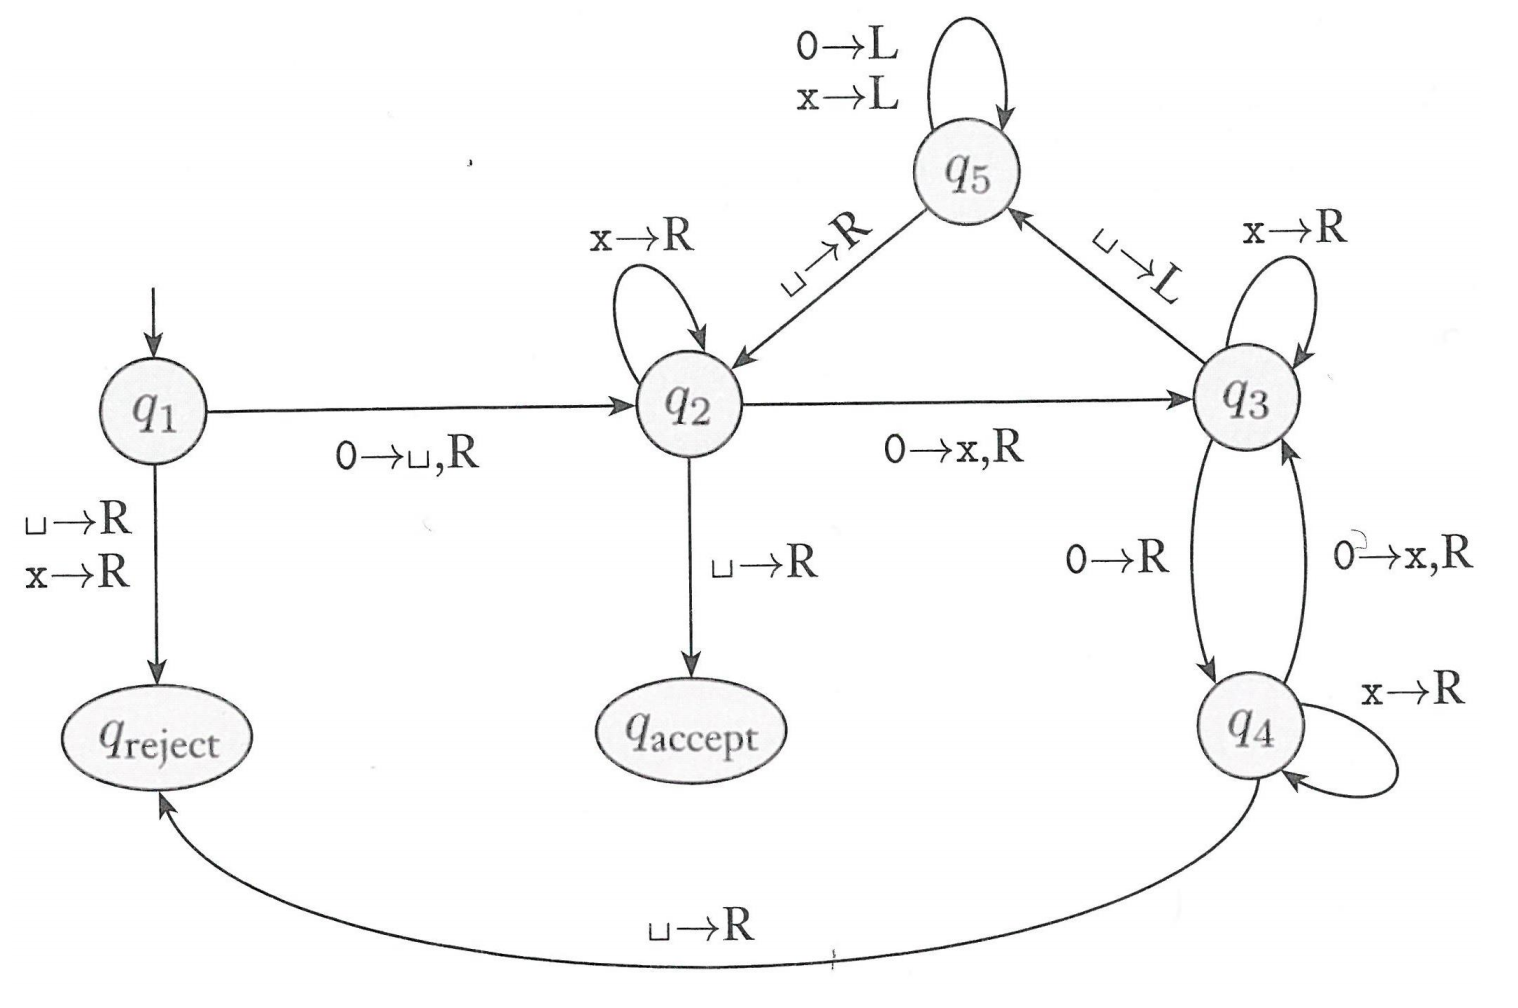
\includegraphics[width=0.7\textwidth]{images/turing-machine-01.png}
        \end{center}
    \item the start, accept, and reject states are $q_1$, $q_\text{accept}$, and $q_\text{reject}$ respectively.
\end{enumerate}
Give the sequence of configurations that $M$ enters when started on the input string
\begin{parts}
    \part $00$;
    \begin{solution}
        In this solution, a configuration will be denoted as \texttt{$q_i$:0\^ 00} where $q_i$ is the state and the hat symbol representing the position of the head on the tape.

    \texttt{$q_1$:\^00, $q_2$:\textvisiblespace\^0, $q_3$:\textvisiblespace x\^\textvisiblespace, $q_5$:\textvisiblespace\^x\textvisiblespace, $q_2$:\^\textvisiblespace x\textvisiblespace, $q_\text{accept}$:\textvisiblespace\^x\textvisiblespace}.
        This exercise is just following a finite state diagram, the other solutions will be omitted.
    \end{solution}

    \part $000$; and
    \part $000000$.
\end{parts}

\question Examine the formal definition of a Turing machine to answer the following questions, and explain your reasoning.
\begin{parts}
    \part Can a Turing machine ever write the blank symbol $\textvisiblespace$ on its tape?
    \begin{solution}
        Yes, look at the Turing machine above.
    \end{solution}

    \part Can the tape alphabet $\Gamma$ be the same as the input alphabet $\Sigma$?
    \begin{solution}
        No, the input alphabet cannot contain the blank character (by definition) and the tape alphabet must satisfy $\textvisiblespace \in \Gamma$ and $\Sigma \subset \Gamma$.
    \end{solution}

    \part Can a Turing machine's head \emph{ever} be in the same location in two succesive steps?
    \begin{solution}
        This kind of depends on your definition of a Turing machine. On uni-directional Turing machines it is typically defined that if you try to move left past the first element on the tape, then the head will stay in the same place. If this is the case, then the answer is yes; however, for bidirectional Turing machines (which is how I like to look at Turing machines) the answer is no.  
    \end{solution}

    \part Can a Turing machine contain just a single state?
    \begin{solution}
        No. In a Turing we have $q_\text{accept} \neq q_\text{reject}$ and they both must exist.
    \end{solution}
\end{parts}

\question Give implementation level descriptions of Turing machines that decide the following languages over the alphabet $\{ 0, 1 \}$:
\begin{parts}
    \part $\{ w : w \;\text{contains an equal number of 0s and 1s} \}$;
    \begin{solution}
        We define a Turing machine that will read the value at the head. If it is the blank symbol it will move right and start again. If it is $1$ or $0$ it will mark it with a blank symbol and move on (but will mark with $x$ instead of the blank symbol from now on). Now the Turing machine will will move right if it is another blank symbol or if it finds the same number it found the first time. If it finds the different number, it will mark it with $x$ then move back to the left where the blank symbol is. From now, if it marks a character it will do it with $x$ and not with the blank character, as that was just used to mark the start point. It will do this until it reaches the end of the tape. If it reaches the end of the tape while looking for a character match, it rejects. Otherwise it accepts.
    \end{solution}

    \part $\{ w : w \;\text{contains twice as many 0s and 1s} \}$; and
    \begin{solution}
        Follows a similar implementation to above; however, if it finds a 1 it will look for two 0s and if it finds a 0 it will look for one 0 and one 1.
    \end{solution}

    \part $\{ w : w \;\text{does not contain twice as many 0s as 1s} \}$.
    \begin{solution}
        We can use the same implementation as above but with the accept and reject states swapped.
    \end{solution}
\end{parts}

\question Give a formal description of a Turing machine that decides the following language over the alphabet $\{ 0, 1 \}$:
\[ \{ w : w \;\text{contains an equal number of 0s and 1s} \}. \] 
\begin{solution}
    \begin{center}
        \begin{tikzpicture}[scale=0.2]
            \tikzstyle{every node}+=[inner sep=0pt]
            \draw [black] (10.1,-17.1) circle (3);
            \draw (10.1,-17.1) node {$q_1$};
            \draw [black] (28.8,-17.1) circle (3);
            \draw (28.8,-17.1) node {$q_2$};
            \draw [black] (10.1,-32.4) circle (3);
            \draw (10.1,-32.4) node {$q_3$};
            \draw [black] (28.8,-32.4) circle (3);
            \draw (28.8,-32.4) node {$q_4$};
            \draw [black] (10.1,-49.1) circle (3);
            \draw (10.1,-49.1) node {$q_\text{reject}$};
            \draw [black] (48.7,-17.1) circle (3);
            \draw (48.7,-17.1) node {$q_\text{reject}$};
            \draw [black] (10.1,-0.7) circle (3);
            \draw (10.1,-0.7) node {$q_\text{accept}$};
            \draw [black] (13.1,-17.1) -- (25.8,-17.1);
            \fill [black] (25.8,-17.1) -- (25,-16.6) -- (25,-17.6);
            \draw (19.45,-17.6) node [below] {$0\to x,R$};
            \draw [black] (10.1,-20.1) -- (10.1,-29.4);
            \fill [black] (10.1,-29.4) -- (10.6,-28.6) -- (9.6,-28.6);
            \draw (9.6,-24.75) node [left] {$1\to x,R$};
            \draw [black] (9.55,-35.337) arc (17.1301:-270.8699:2.25);
            \draw (3.07,-38.3) node [below] {$1\to R$};
            \fill [black] (7.43,-33.75) -- (6.52,-33.51) -- (6.82,-34.46);
            \draw [black] (31.387,-33.896) arc (87.69007:-200.30993:2.25);
            \draw (36.96,-38.52) node [below] {$0,1,x\to L$};
            \fill [black] (29.19,-35.36) -- (28.65,-36.14) -- (29.65,-36.18);
            \draw [black] (26.48,-30.5) -- (12.42,-19);
            \fill [black] (12.42,-19) -- (12.72,-19.89) -- (13.36,-19.12);
            \draw (28.59,-24.26) node [above] {\textvisiblespace$\to R$};
            \draw [black] (7.137,-16.714) arc (290.30993:2.30993:2.25);
            \draw (3.87,-12.02) node [left] {$x\to R$};
            \fill [black] (8.6,-14.51) -- (8.8,-13.59) -- (7.86,-13.94);
            \draw [black] (10.1,-35.4) -- (10.1,-46.1);
            \fill [black] (10.1,-46.1) -- (10.6,-45.3) -- (9.6,-45.3);
            \draw (9.6,-40.75) node [left] {\textvisiblespace$\to R$};
            \draw [black] (31.8,-17.1) -- (45.7,-17.1);
            \fill [black] (45.7,-17.1) -- (44.9,-16.6) -- (44.9,-17.6);
            \draw (38.75,-17.6) node [below] {\textvisiblespace$\to R$};
            \draw [black] (10.1,-14.1) -- (10.1,-3.7);
            \fill [black] (10.1,-3.7) -- (9.6,-4.5) -- (10.6,-4.5);
            \draw (10.6,-8.9) node [right] {\textvisiblespace$\to R$};
        \end{tikzpicture}
    \end{center}
\end{solution}

\question
\begin{parts}
    \part Show that the collection of decidable languages is closed under the operation of union.
    \begin{solution}
        If we have the union of $n$ decidable languages. Then we can construct a $n$-tape Turing machine which will run the corresponding Turing machine for each one. As each language is decidable, they will all terminate; hence, the multi-tape will also terminate. Therefore, the collection of decidable languages is closed under union. 
    \end{solution}

    \part Show that the collection of Turing-recognisable languages is closed under the operation of union.
    \begin{solution}
        Following a similar logic from last part with the $n$-tape Turing machine; however, some tapes may not terminate. This does not matter however as we just need to be Turing-recognisable and not Turing-decidable. As long as the tapes are ran in parallel, the tape the accepts an input will eventually terminate. If none of the Turing machines accept an input and one of them does not terminate then the multitape Turing machine will never terminate. 
    \end{solution}
\end{parts}

\question A \emph{Turing machine with left reset} is similar to an ordinary Turing machine, but the transition function has the form
\[ \delta: Q \times \Gamma \to Q \times \Gamma \times \{R, RESET\}. \]
If 
$\delta(q, a) = (r, b, RESET)$,
when the machine is in state $q$ reading an $a$, the machine's head jumps to the left-hand end of the tape after it writes $b$ on the tape and enters state $r$. Note that these machines do not have the usual ability to move the head one symbol left. Show that Turing machines with left reset recognise the class of Turing-recognisable languages.
\begin{solution}
    It is enough for us to show that if we can replicate a left move with this Turing machine then it recognises the class of Turing-recognisable languages. So, to move left:
    \begin{enumerate}
        \item dot the current cell, reset to the first cell;
        \item dot the first cell, move right and dot the cell, reset;
        \item move right until you hit a dot then erase it, move right two;
        \item if the cell is dotted then erase it and reset and move right until you hit a dot, you are now left;
        \item if the cell is not dotted then dot it.
    \end{enumerate}
    Hence Turing machines with left reset recognise the class of Turing-recognisable languages. What more, it also decides the class of decidable languages.
\end{solution}
